%\newcommand{\MADGRAPH} {\textsc{MadGraph}\xspace}
%\newcommand{\MCATNLO} {\textsc{mc@nlo}\xspace}
%\newcommand{\MGvATNLO }{\MADGRAPH{}5\_a\MCATNLO}
%\newcommand{\PYTHIA} {{\textsc{pythia}}\xspace}
%\newcommand{\GEANTfour} {{\textsc{Geant4}}\xspace}
%\newcommand{\kt}{\ensuremath{k_{\mathrm{T}}}\xspace}
%\newcommand{\abs}[1]{\ensuremath{\lvert #1 \rvert}}

%\newcommand{\abinv} {\mbox{\ensuremath{\,\text{ab}^\text{$-$1}}}\xspace}


%\newcommand{\Hbb}{\ensuremath{ H \to b\bar{b} }\xspace}
%\newcommand{\ttjets}{\ttbar+jets\xspace}
%\newcommand{\intLumi}{3\abinv}
%\newcommand{\MJJ}{\ensuremath{m_{\text{JJ}}}\xspace}
%\newcommand{\mjj}{\ensuremath{m_{\text{jj}}}\xspace}
%\newcommand{\mH}{\ensuremath{m_{ H }}\xspace}
%\newcommand{\nsub}{\ensuremath{\tau_{21}}\xspace}
%\newcommand{\mjone}{\ensuremath{m_{\text{j}_{1}}}\xspace}
%\newcommand{\mjtwo}{\ensuremath{m_{\text{j}_{2}}}\xspace}
%\newcommand{\LambdaR}{\ensuremath{\Lambda_{\text{R}}}\xspace}
%\newcommand{\DeltaEta}{\ensuremath{\Delta\eta(\text{j}_{1}, \text{j}_{2})}\xspace}
%\newcommand{\mx}{\ensuremath{m_{ X }}\xspace}
%\newcolumntype{P}[1]{>{\centering\arraybackslash}p{#1}}


\subsubsection{\cmsC{Search for VBF production of resonances decaying to HH in the 4b final state with large radius jet substructure}}
\contributors{J. Komaragiri, D. Majumder, A. Carvalho, L. Panwar, CMS}\rt{There are comments to address. I have serious doubts on the validity of this analysis.}
%{\bf Author(s): J. Komaragiri, D. Majumder, A. Carvalho, L. Panwar, CMS}

Several beyond standard model (BSM) scenarios predict the existence of resonances decaying to a pair of Higgs bosons, $ H $~\cite{HiggsDiscoveryAtlas,HiggsDiscoveryCMS,CMSHiggsLongPaper}, such as warped extra dimensional (WED) models~\cite{Randall:1999ee}, which have a spin-0 
radion~\cite{Goldberger:1999uk,Csaki:1999mp,Csaki:2000zn} and a spin-2 first Kaluza--Klein (KK) excitation of the graviton~\cite{Davoudiasl:1999jd,DeWolfe:1999cp, Agashe:2007zd}. 
Others, such as the two-Higgs doublet models~\cite{Branco:2011iw} 
(particularly, the MSSM~\cite{Djouadi:2005gj}) and the Georgi-Machacek model~\cite{GEORGI1985463} also contain spin-0 
resonances. 
These resonances may have a sizeable branching fraction to a Higgs pair.

Searches for a new particle $X$ in the $HH$ decay channel have been performed by the
ATLAS~\cite{Aad:2014yja, Aad:2015uka, Aad:2015xja} and
CMS~\cite{Khachatryan:2014jya, Khachatryan:2015year, Khachatryan:2015tha,Khachatryan:2016sey,Khachatryan:2016cfa}
Collaborations in proton-proton ($ p  p $) collisions at $\sqrt{s} =  7$ and 8\TeV.
The ATLAS Collaboration has set limits on the production of a KK bulk graviton decaying to $HH$ in the final state with a pair of $ b $ quark and antiquark, $ b\bar{b}  b\bar{b} $, using $ p  p $ collision data at $\sqrt{s} = 13\TeV$~\cite{Aaboud:2016xco,ATLAS-CONF-2016-049,Aaboud:2018knk}.
The CMS Collaboration has also set limits on the production of a KK bulk graviton and a radion, decaying to $HH$, in the $ b\bar{b}  b\bar{b} $ final state, using $ p  p $ collision data at $\sqrt{s} = 13\TeV$, corresponding to an integrated luminosity of 35.9\fbinv~\cite{CMS-B2G-16-026,CMS-B2G-17-019}. 
At present, the searches from ATLAS and CMS set a limit on the production cross sections and the branching fractions $\sigma( p  p  \to  X ) \mathcal{B}( X  \to  H  H  \to  b\bar{b}   b\bar{b} )$ for masses of $X$, $m_{X}$ up to 3000\GeV.

The searches were confined to the $s$-channel production of a narrow resonance $X$ from the standard model (SM) quark-antiquark or gluon-gluon interactions. 
The WED models that were used in the interpretations of the results have extra spatial dimension compactified between two branes (called the bulk) via an exponential metric ${\kappa l}$, where $\kappa$ is the warp factor and $l$ the coordinate of the extra spatial dimension~\cite{Giudice:2000av}. 
The reduced Planck scale, $\overline{\Mpl} \equiv \Mpl/8\pi$, \Mpl being the Planck scale and the ultraviolet cutoff of the theory $\LambdaR \equiv \sqrt{6} e^{-\kappa l} \overline{\Mpl}$~\cite{Goldberger:1999uk} are fundamental scales in these models.
The cross section limit of a bulk graviton decaying to $ H  H  \to  b\bar{b}   b\bar{b} $ is between 4 and 1.4\unit{fb} for masses between 1400 and 3000\GeV, while a radion of mass below 1400\GeV\ is excluded at 95\%~\cl for $\LambdaR = 3\TeV$~\cite{CMS-B2G-16-026}.

The searches for these resonances in other production modes, such as VBF, as depicted in \fig{fig_tdr:feyn}, has not yet been explored.
While the $s$-channel production cross section of a bulk graviton, assuming $\kappa/\overline{\Mpl} = 0.5$, is in the range 5--0.05\unit{fb} for masses between 1500 and 3000\GeV, the VBF production mode is expected to have a cross section an order of magnitude smaller~\cite{TheoryReview}.
The absence of a signal from the $s$-channel process may point to highly suppressed couplings of $X$ with the SM quarks and gluons, making VBF the dominant production process in $ p  p $ collisions.
 
%The VBF production process $ p  p \to X \Pq\Paq$ should be observable at HL-LHC.

\begin{figure}[htbp]
  \begin{center}
    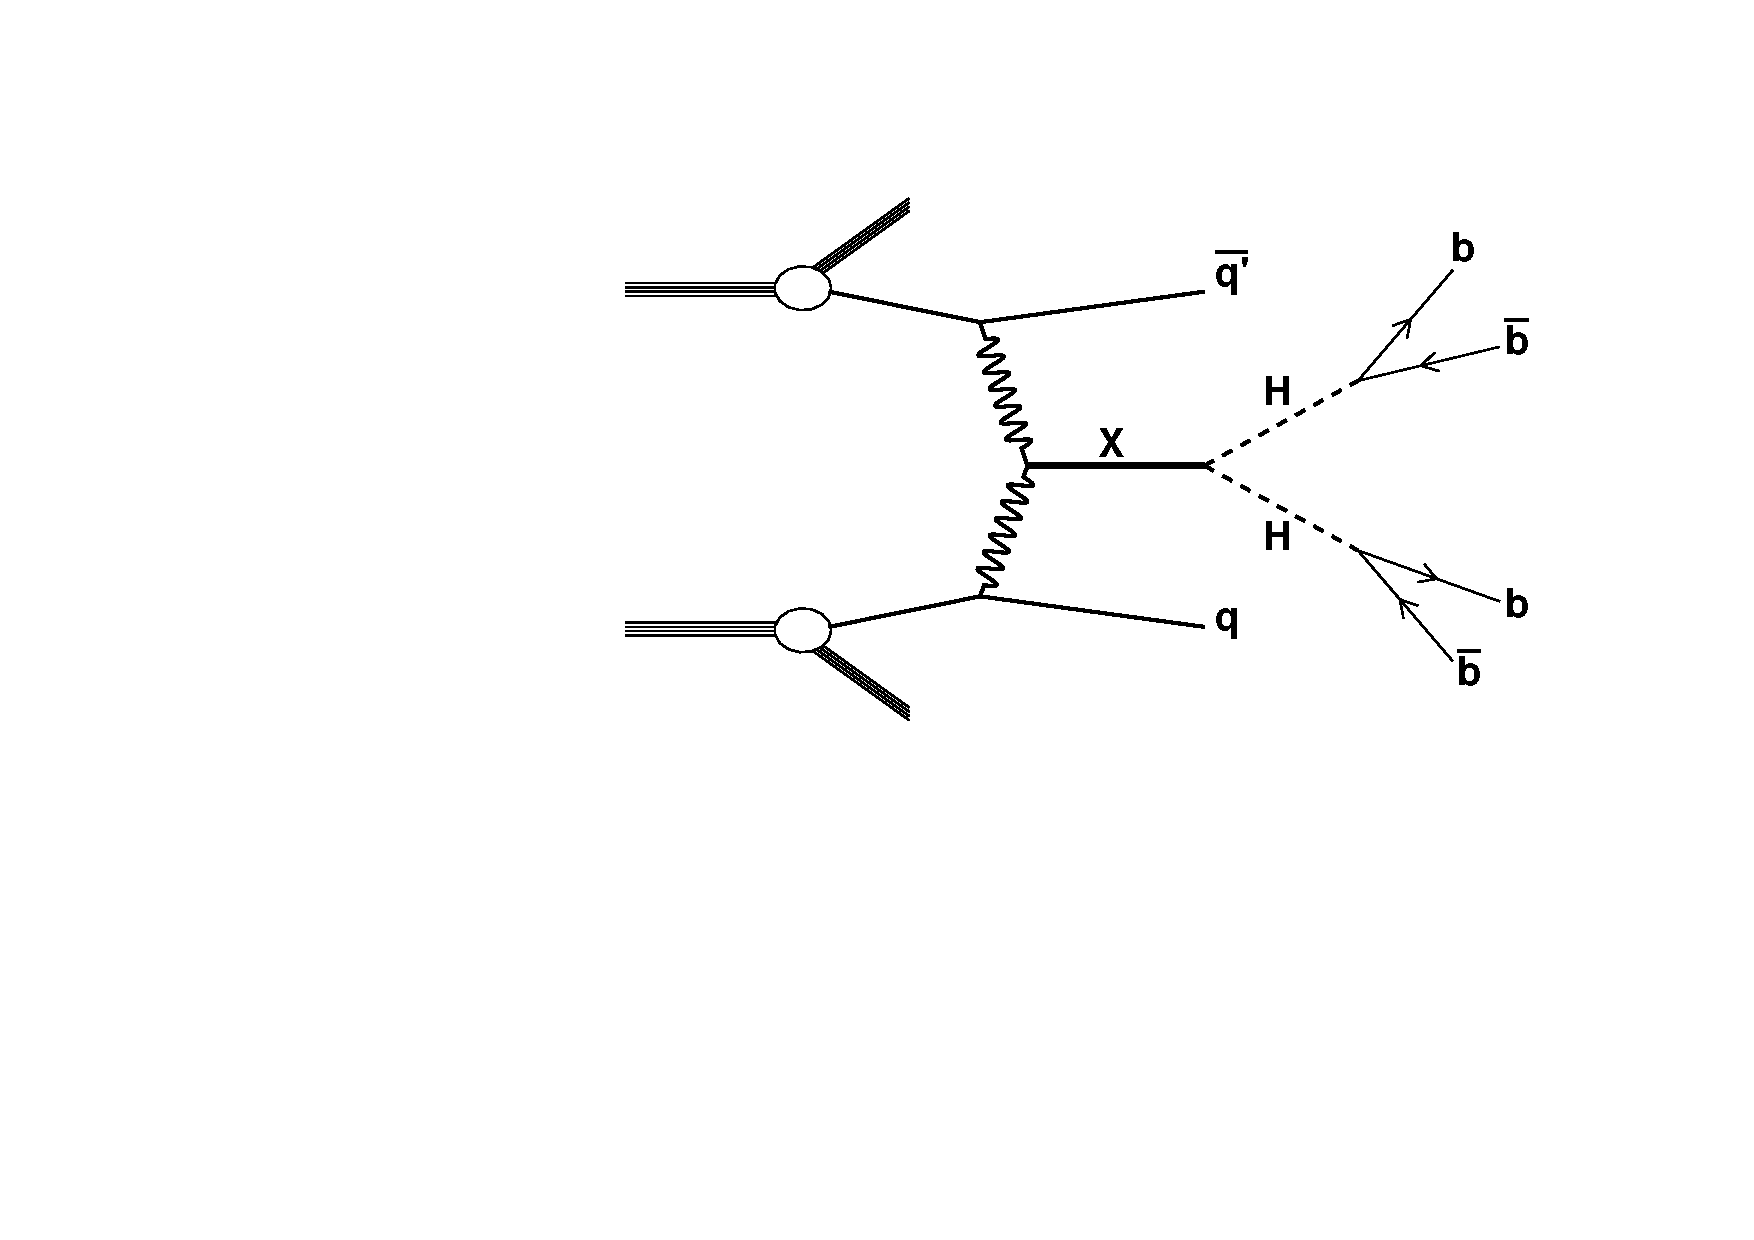
\includegraphics[width=0.495\textwidth]{\main/section7OtherSignatures/img/vbfhhres.pdf}
    \caption{The vector boson fusion mode of production of a resonance $X$ decaying to a pair of Higgs bosons $ H $, with both Higgs bosons decaying to $ b\bar{b} $ pairs.}
    \label{fig_tdr:feyn}
  \end{center}
\end{figure}

Here we explore the prospects for the search for a massive resonance produced through VBF and decaying to $HH$ at the HL-LHC with the upgraded CMS detector. For a very massive resonance, highly Lorentz-boosted Higgs bosons are more efficiently reconstructed as a large-area jet (Higgs jet). In addition, a signal event will also have two energetic jets at large pseudorapidity $\eta$. This study is reported in detail in \citeref{CMS-PAS-FTR-18-003}


A simulation of the upgraded Phase 2 CMS detector was used for this study. 
Signal events for bulk gravitons were simulated at leading order using {\MGvATNLO  2.4.2}~\cite{MG5_aMCNLO} for 
masses in the range 1500--3000\GeV and for a fixed width of 1\% of the mass. The {NNPDF3.0} leading order PDFs~\cite{Ball:2014uwa}, taken from the {LHAPDF6} PDF set~\cite{Harland-Lang:2014zoa,Buckley:2014ana,Carrazza:2015hva,Butterworth:2015oua}, with the four-flavour scheme, were used. The main background is given by multijet events, and has been simulated using \PYTHIA~8.212~\cite{Pythia8p2}, for events containing two hard partons, with the invariant mass of the two partons required to be greater than 1000 GeV.

For both the signal and the background processes, the showering and hadronization of partons was simulated with \PYTHIA~8. 
The pileup events contribute to the overall event activity in the detector, the effect of which was included in the simulations assuming a pileup distribution averaging to 200.
All generated samples were processed through a \GEANTfour-based~\cite{Agostinelli:2002hh,GEANT} simulation of the upgraded CMS detector.

The two leading-$\pt$ AK8 jets in the event, $J_{1}$ and $J_{2}$, are required to have $\pt > 300\GeV$ and  $\abs{\eta} < 3.0$. To identify the two leading-$\pt$ AK8 jets with the boosted $H\to b\bar{b}$ candidates from the $ X \to H  H $ decay ($ H $ tagging), these jets are groomed~\cite{Salam:2009jx} to remove soft and wide-angle radiation using the modified mass drop algorithm~\cite{Butterworth:2008iy,Dasgupta:2013ihk}, with the soft radiation fraction parameter $z$ set to $0.1$ and the angular exponent parameter $\beta$ set to 0, also known as the soft-drop algorithm~\cite{Larkoski:2014wba,CMS-PAS-JME-16-003}.
By undoing the last stage of the jet clustering, one gets two subjets each for $J_{1}$ and $J_{2}$.
The invariant mass of the two subjets is the soft-drop mass of each AK8 jet, which has a distribution with a peak near the Higgs boson mass $m_{H}$ = 125 GeV~\cite{Aad:2015zhl,Sirunyan:2017exp}, and a width of about 10\%.
The soft-drop mass window selection was optimized using a figure of merit of $S/\sqrt{B}$ and required to be in the range 90--140 GeV for both leading jets.

The $N$-subjettiness ratio $\nsub \equiv \tau_2/\tau_1$ has a value much smaller than unity for a jet with two subjets. For signal selection, $J_{1}$ and $J_{2}$ are required to have $\nsub < 0.6$ following an optimization of the above figure of merit.

The $ H $ tagging of $J_{1}$ and $J_{2}$ further requires identifying their subjet pairs to be $ b $ tagged with a probability of about 49\% to contain at least one $ b $ hadron, and a corresponding probability of about 1\% of having no $ b $ or $\Pqc$ hadrons. 
Events are classified into two categories: those having exactly three out of the four $ b $-tagged subjets ($3 b $ category), and those that have all four subjets $ b $-tagged ($4 b $ category).

Events are required to have at least two AK4 jets $j_{1}$ and $j_{2}$, which are separated from the $ H $ jets by $\Delta R> 1.2$, with $\pt > 50\GeV$ and $\abs{\eta}< 5$.
To pass the VBF selections, these jets must lie in opposite $\eta$ regions of the detector, and a pseudorapidity difference $\abs{\Delta\eta(j_{1}, j_{2})} > 5$.
The invariant mass $m_{jj}$ reconstructed using these AK4 jets is required to pass $m_{jj} > 300$ GeV.

The bulk graviton invariant mass $M_{JJ}$ is reconstructed from the 4-momenta of the two Higgs jets in events passing the above mentioned full selection criteria. The main multijet background is smoothly falling, above which the signal is searched for, as a localized excess of events, for a narrow resonance $X$. 

It is expected that the multijet background component in a true search at the HL-LHC will rely on the data for a precise estimate. Methods such as those described in \citeref{CMS-B2G-16-026} are known to provide an accurate prediction of the multijet background $M_{JJ}$ shape as well as the yield. 
%Here, the expected background yields based on simulations are described. 

The simulated multijet background sample consists of $\sim\!4$ million events none of which survive the full selection. To estimate the background, the subjet $ b $-tagging efficiency is determined using a loose set of selections which require events to have $J_{1}$ and $J_{2}$ passing only the soft-drop mass and $\nsub$ requirements. The $ b $-tagging efficiency is obtained for the different subjet flavours and as a function of $\pt$ and $\eta$. 

Multijet events passing all selections but the subjet $ b $ tagging are then reweighted according to the subjet efficiencies to obtain the probability of the event to pass the three of four subjet $ b $-tagging categories. The $M_{JJ}$ distributions for the multijet background after the full selection are then obtained from the weighted events in these two categories. 

From the analysis of current LHC data at $\sqrt{s} = 13\TeV$, it was found that the multijet backgrounds in simulations is overestimated by a factor of 0.7 compared to the yields in the data. \rt{What does it mean overestimated by a factor 0.7?} Accordingly, the multijet background yield has been corrected by this factor, assuming this to hold also for the simulations of the multijet processes at $\sqrt{s} = 14\TeV$ .
The $M_{JJ}$ of the backgrounds thus obtained and the signals are shown in \fig{fig:MJJ}, while the event yields after full selection are given in \tabb{tab:evtyields}. 

The efficiency of events to pass the VBF jet selection depends strongly on pileup due to the combinatorial backgrounds from pileup jets, which affects both the signal and the background selection. Moreover, the VBF selection efficiency for multijets grows faster than the signal efficiency with pileup, since the latter has true VBF jets which already pass the selection in the absence of pileup. Hence, in the present search, the requirement of additional VBF jets does not result in any appreciable gain in the signal sensitivity. It is anticipated that developments in the rejection of pileup jets in the high $\eta$ region will eventually help suppress the multijets background and improve the signal sensitivity further.

\begin{figure}[tbp]
  \begin{center}
    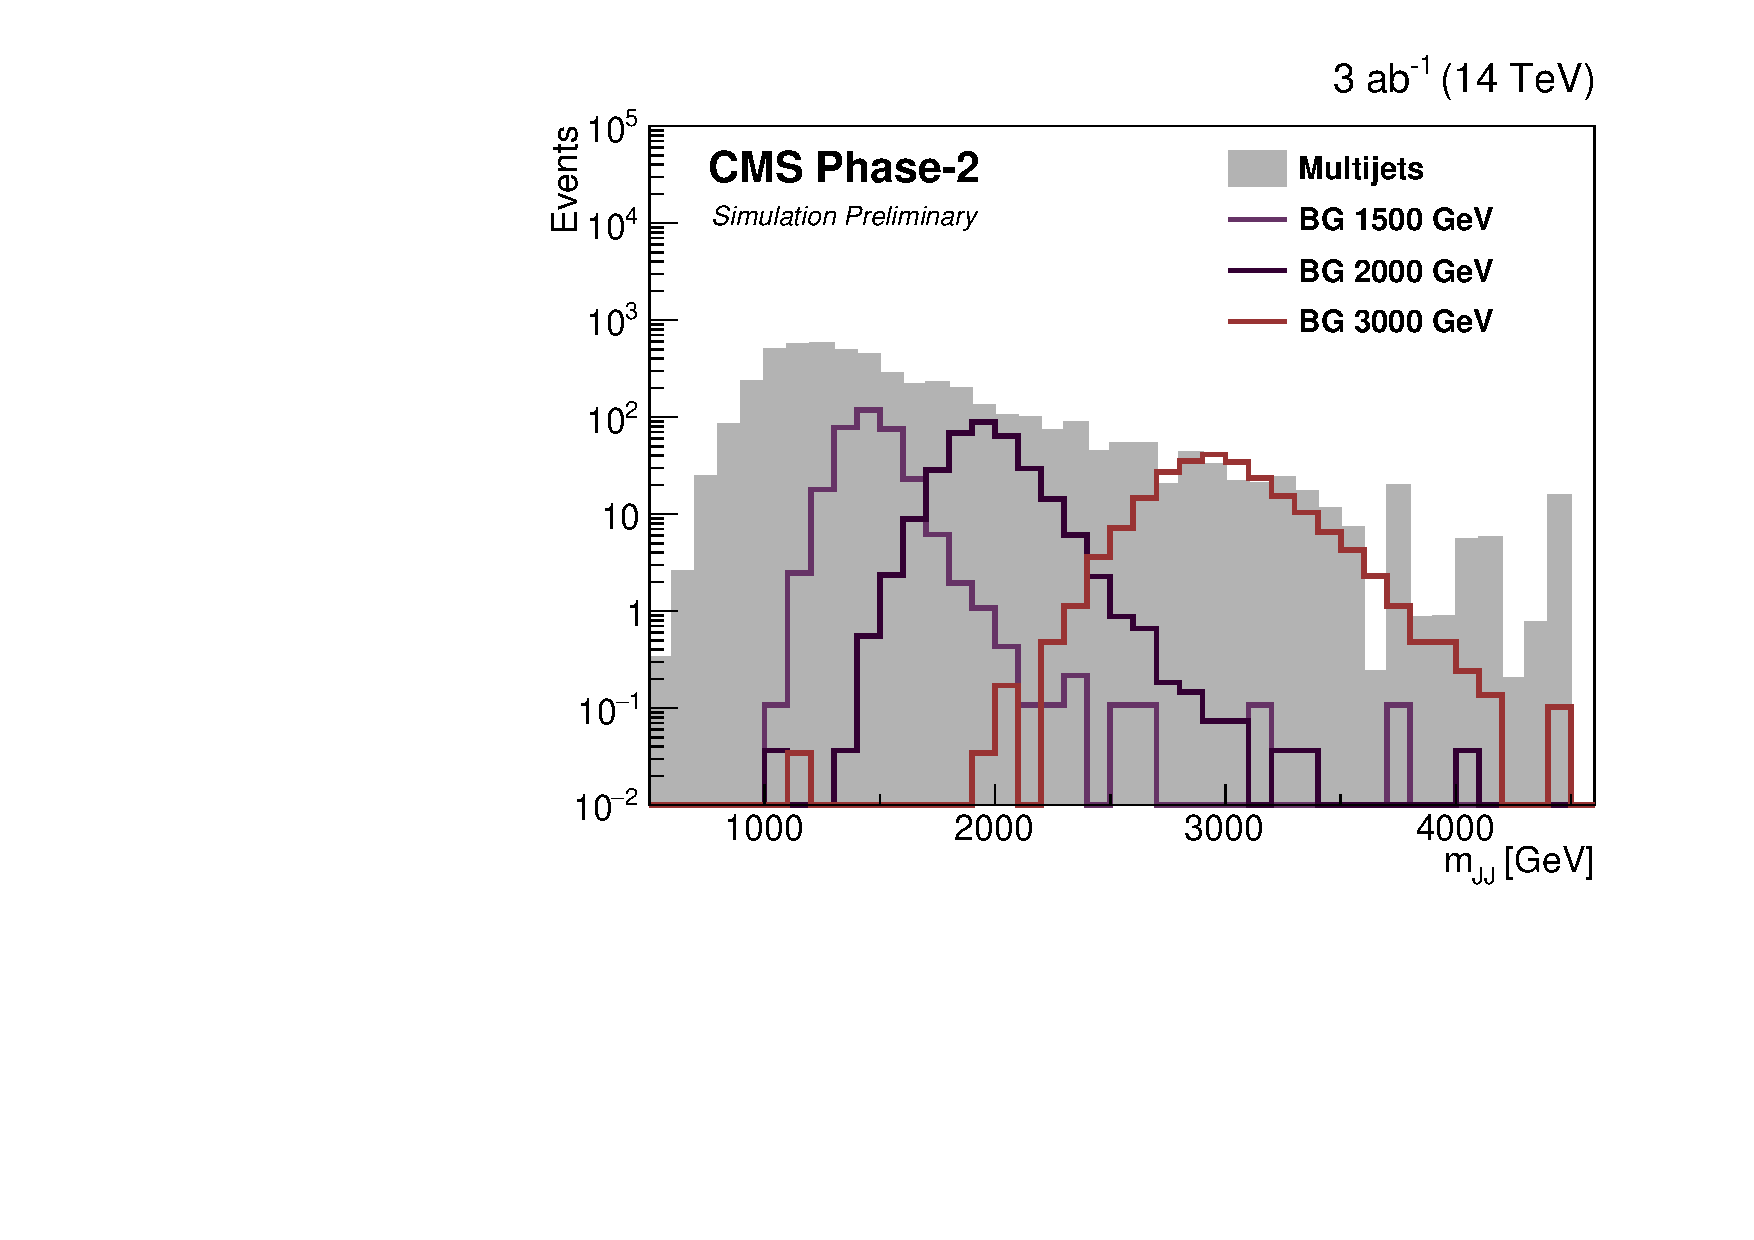
\includegraphics[width=0.495\textwidth]{\main/section7OtherSignatures/img/c_compare_h_mjj_3b_200_Logy1.pdf}
    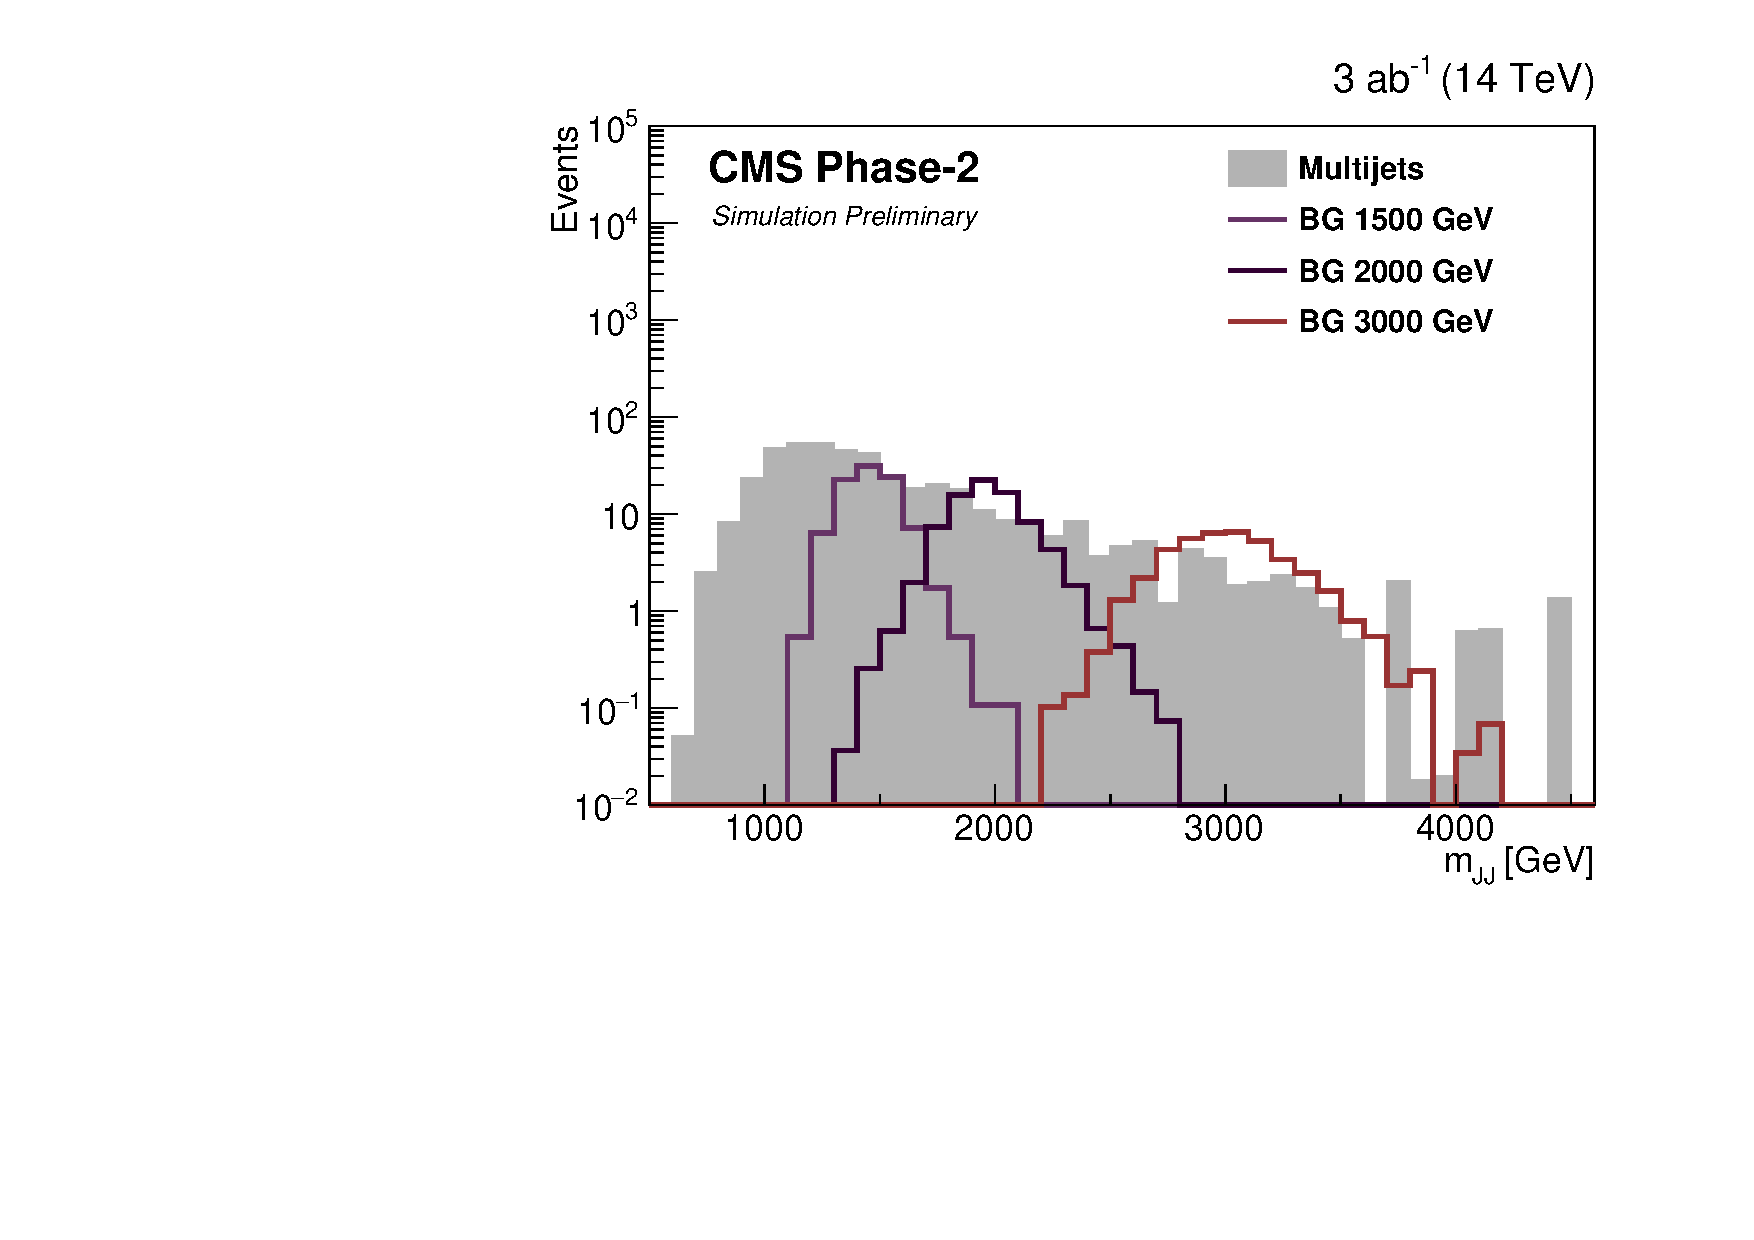
\includegraphics[width=0.495\textwidth]{\main/section7OtherSignatures/img/c_compare_h_mjj_4b_200_Logy1.pdf}
    \caption{The estimated multijet background and the signal $\mjj$ distributions for bulk gravitons (BG) of masses 1500, 2000, and 3000\GeV, assuming a signal cross section of 1\unit{fb}. The distributions on the left are for the $3 b $ and those on the right are for the $4 b $ subjet $ b $-tagged categories and for an average pileup of 200.}
    \label{fig:MJJ}
  \end{center}
\end{figure}

\begin{table}
  \begin{center}
    \caption{Event yields and efficiencies for the signal and multijet background for an average pileup of 200. The product of the cross sections and branching fractions of the signals $\sigma( p  p  \to  X \text{jj} \to  H  H  \text{jj})$ is assumed to be 1\unit{fb}. Owing to the large sample sizes of the simulated events, the statistical uncertainties are small.}\label{tab:evtyields}
    \begin{tabular}{ccccc}
      \hline\hline
      Process & \multicolumn{2}{c}{$3 b $ category} & \multicolumn{2}{c}{$4 b $ category} \\ \hline
                                  & Events & Efficiency (\%)     & Events & Efficiency (\%) \\ \hline 
      Multijets                   & 4755   & $1.6\times 10^{-3}$ & 438    & $1.5\times 10^{-4}$ \\ 
      BG (\mx=1500\GeV) & 326    & 11                  & 95.2   & 3.2\\ 
      BG (\mx=2000\GeV) & 316    & 11                  & 81.2   & 2.7\\ 
      BG (\mx=3000\GeV) & 231    & 7.7                 & 41.4   & 1.4\\ 
      \hline\hline
    \end{tabular}
  \end{center}
\end{table}

The expected significance of the signal, assuming a production cross section of 1\unit{fb} is estimated. Several systematic uncertainties are considered.\rt{Inconsistent assumption.}
The uncertainty in the jet energy scale amounts to 1\%. The uncertainty in the subjet $ b $-tagging efficiency difference between the data and simulations is taken to be 1\%. An uncertainty of 1\% is assigned to the integrated luminosity measurement. These uncertainties are based on the projected values for the full data set at the HL-LHC.

In addition, several measurement uncertainties are considered based on the 2016 search for a resonance decaying to a pair of boosted Higgs bosons~\cite{CMS-B2G-16-026}, scaled by 0.5. 
The $ H $ jet selection uncertainties include the uncertainties in the $ H $ jet mass scale and resolution (1\%), the uncertainty in the data to simulation difference in the selection on \nsub (13\%), and the uncertainty in the showering and hadronization model for the $ H $ jet (3.5\%). 
The uncertainties in the signal acceptance because of the parton distribution functions (1\%) and the simulation of the pileup (1\%) are also taken into account

The expected signal significance of a bulk graviton of mass between 1500 and 3000\GeV, produced through vector boson fusion, and decaying into a pair of Higgs bosons, each of which decays to a  $b\bar{b}$ pair, is given in \fig{fig:sigSig} for an integrated luminosity of \intLumi.\rt{The significance cannot grow with the mass (i.e.~the cross section cannot be kept fixed),}

\begin{figure}[htbp]
  \begin{center}
    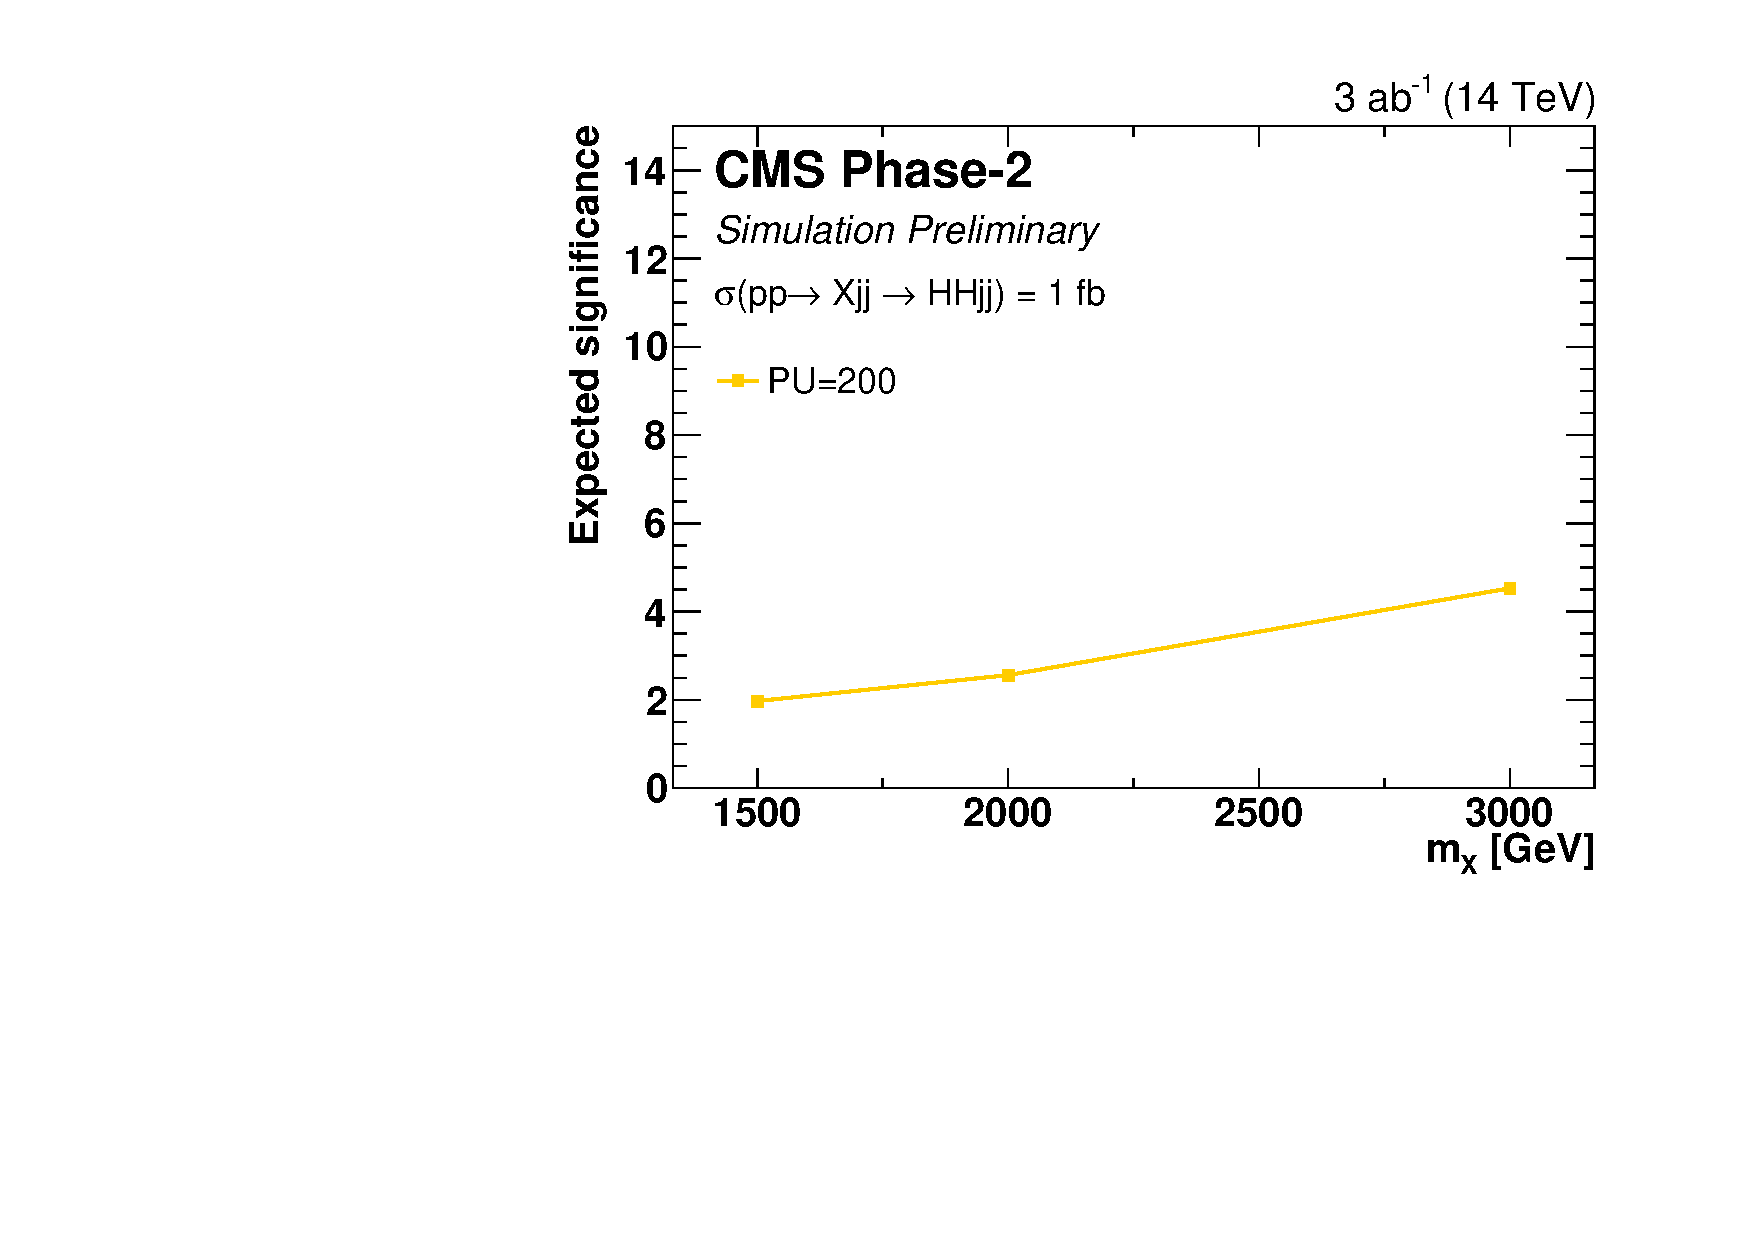
\includegraphics[width=0.5\textwidth]{\main/section7OtherSignatures/img/Significance_WPM.pdf}
    \caption{Expected signal significance for Bulk Gravitons of masses 1500, 2000, and 3000\GeV, assuming a production cross section of 1\unit{fb}. The data set corresponds to an integrated luminosity of \intLumi and with a pileup of 200.}
    \label{fig:sigSig}
  \end{center}
\end{figure}








